\documentclass{article}\usepackage[]{graphicx}\usepackage[]{color}
% maxwidth is the original width if it is less than linewidth
% otherwise use linewidth (to make sure the graphics do not exceed the margin)
\makeatletter
\def\maxwidth{ %
  \ifdim\Gin@nat@width>\linewidth
    \linewidth
  \else
    \Gin@nat@width
  \fi
}
\makeatother

\definecolor{fgcolor}{rgb}{0.345, 0.345, 0.345}
\newcommand{\hlnum}[1]{\textcolor[rgb]{0.686,0.059,0.569}{#1}}%
\newcommand{\hlstr}[1]{\textcolor[rgb]{0.192,0.494,0.8}{#1}}%
\newcommand{\hlcom}[1]{\textcolor[rgb]{0.678,0.584,0.686}{\textit{#1}}}%
\newcommand{\hlopt}[1]{\textcolor[rgb]{0,0,0}{#1}}%
\newcommand{\hlstd}[1]{\textcolor[rgb]{0.345,0.345,0.345}{#1}}%
\newcommand{\hlkwa}[1]{\textcolor[rgb]{0.161,0.373,0.58}{\textbf{#1}}}%
\newcommand{\hlkwb}[1]{\textcolor[rgb]{0.69,0.353,0.396}{#1}}%
\newcommand{\hlkwc}[1]{\textcolor[rgb]{0.333,0.667,0.333}{#1}}%
\newcommand{\hlkwd}[1]{\textcolor[rgb]{0.737,0.353,0.396}{\textbf{#1}}}%
\let\hlipl\hlkwb

\usepackage{framed}
\makeatletter
\newenvironment{kframe}{%
 \def\at@end@of@kframe{}%
 \ifinner\ifhmode%
  \def\at@end@of@kframe{\end{minipage}}%
  \begin{minipage}{\columnwidth}%
 \fi\fi%
 \def\FrameCommand##1{\hskip\@totalleftmargin \hskip-\fboxsep
 \colorbox{shadecolor}{##1}\hskip-\fboxsep
     % There is no \\@totalrightmargin, so:
     \hskip-\linewidth \hskip-\@totalleftmargin \hskip\columnwidth}%
 \MakeFramed {\advance\hsize-\width
   \@totalleftmargin\z@ \linewidth\hsize
   \@setminipage}}%
 {\par\unskip\endMakeFramed%
 \at@end@of@kframe}
\makeatother

\definecolor{shadecolor}{rgb}{.97, .97, .97}
\definecolor{messagecolor}{rgb}{0, 0, 0}
\definecolor{warningcolor}{rgb}{1, 0, 1}
\definecolor{errorcolor}{rgb}{1, 0, 0}
\newenvironment{knitrout}{}{} % an empty environment to be redefined in TeX

\usepackage{alltt}
\IfFileExists{upquote.sty}{\usepackage{upquote}}{}
\begin{document}



Load the necessary libraries:
\begin{knitrout}
\definecolor{shadecolor}{rgb}{0.969, 0.969, 0.969}\color{fgcolor}\begin{kframe}
\begin{alltt}
\hlkwd{library}\hlstd{(ggplot2)}
\hlkwd{library}\hlstd{(MCMCpack)}
\end{alltt}


{\ttfamily\noindent\color{warningcolor}{\#\# Warning: package 'MCMCpack' was built under R version 4.0.3}}

{\ttfamily\noindent\itshape\color{messagecolor}{\#\# Loading required package: coda}}

{\ttfamily\noindent\color{warningcolor}{\#\# Warning: package 'coda' was built under R version 4.0.3}}

{\ttfamily\noindent\itshape\color{messagecolor}{\#\# Loading required package: MASS}}

{\ttfamily\noindent\itshape\color{messagecolor}{\#\# \#\#\\\#\# \#\# Markov Chain Monte Carlo Package (MCMCpack)}}

{\ttfamily\noindent\itshape\color{messagecolor}{\#\# \#\# Copyright (C) 2003-2021 Andrew D. Martin, Kevin M. Quinn, and Jong Hee Park}}

{\ttfamily\noindent\itshape\color{messagecolor}{\#\# \#\#\\\#\# \#\# Support provided by the U.S. National Science Foundation}}

{\ttfamily\noindent\itshape\color{messagecolor}{\#\# \#\# (Grants SES-0350646 and SES-0350613)\\\#\# \#\#}}\begin{alltt}
\hlkwd{library}\hlstd{(gridExtra)}
\end{alltt}
\end{kframe}
\end{knitrout}

\section{K=2 source populations}

Figure out how likely Case I, Case II, Case III are

\begin{knitrout}
\definecolor{shadecolor}{rgb}{0.969, 0.969, 0.969}\color{fgcolor}\begin{kframe}
\begin{alltt}
\hlstd{nrSims} \hlkwb{<-} \hlnum{10000}
\hlstd{Jall} \hlkwb{<-} \hlnum{2}\hlopt{:}\hlnum{50} \hlcom{##number of alleles}
\hlstd{alphaBarAll} \hlkwb{<-} \hlnum{1} \hlcom{##common concentration parameter for symmetric multivariate}
\hlcom{##Dirichlet distribution}

\hlstd{fractCaseI} \hlkwb{<-} \hlstd{fractCaseII} \hlkwb{<-} \hlstd{fractCaseIII} \hlkwb{<-}
  \hlkwd{matrix}\hlstd{(}\hlnum{NA}\hlstd{,} \hlkwc{nrow}\hlstd{=}\hlkwd{length}\hlstd{(Jall),} \hlkwc{ncol}\hlstd{=}\hlkwd{length}\hlstd{(alphaBarAll))}

\hlkwd{set.seed}\hlstd{(}\hlnum{380183}\hlstd{)}

\hlkwa{for}\hlstd{(a} \hlkwa{in} \hlnum{1}\hlopt{:}\hlkwd{length}\hlstd{(alphaBarAll))}
\hlstd{\{}
  \hlstd{alphaBar} \hlkwb{<-} \hlstd{alphaBarAll[a]}

  \hlkwd{print}\hlstd{(}\hlstr{"%%%%%%%%%"}\hlstd{)}
  \hlkwd{print}\hlstd{(alphaBar)}
  \hlkwd{print}\hlstd{(}\hlstr{"%%%%%%%%%"}\hlstd{)}

  \hlkwa{for}\hlstd{(J} \hlkwa{in} \hlstd{Jall)}
    \hlstd{\{}
      \hlkwa{if}\hlstd{(J} \hlopt \hlnum{10} \hlopt{==} \hlnum{0}\hlstd{)}
        \hlstd{\{}
          \hlkwd{print}\hlstd{(J)}
        \hlstd{\}}

      \hlstd{cases} \hlkwb{<-} \hlkwd{rep}\hlstd{(}\hlstr{""}\hlstd{, nrSims)}
      \hlkwa{for}\hlstd{(sim} \hlkwa{in} \hlnum{1}\hlopt{:}\hlstd{nrSims)}
      \hlstd{\{}
        \hlcom{##generate some data }
        \hlstd{p1} \hlkwb{<-} \hlkwd{rdirichlet}\hlstd{(}\hlnum{1}\hlstd{,} \hlkwd{rep}\hlstd{(alphaBar, J))}
        \hlstd{p2} \hlkwb{<-} \hlkwd{rdirichlet}\hlstd{(}\hlnum{1}\hlstd{,} \hlkwd{rep}\hlstd{(alphaBar, J))}

        \hlstd{E1} \hlkwb{<-} \hlkwd{sum}\hlstd{(p1}\hlopt{^}\hlnum{2}\hlstd{)}
        \hlstd{E2} \hlkwb{<-} \hlkwd{sum}\hlstd{(p2}\hlopt{^}\hlnum{2}\hlstd{)}
        \hlstd{E12} \hlkwb{<-} \hlkwd{sum}\hlstd{(p1}\hlopt{*}\hlstd{p2)}

        \hlkwa{if}\hlstd{(E1} \hlopt{>} \hlstd{E12} \hlopt{&} \hlstd{E12} \hlopt{>} \hlstd{E2)}
          \hlstd{\{}
            \hlstd{cases[sim]} \hlkwb{<-} \hlstr{"Case I"}
          \hlstd{\}} \hlkwa{else} \hlstd{\{}
            \hlkwa{if}\hlstd{(E2} \hlopt{>} \hlstd{E12} \hlopt{&} \hlstd{E12} \hlopt{>} \hlstd{E1)}
              \hlstd{\{}
                \hlstd{cases[sim]} \hlkwb{<-} \hlstr{"Case II"}
              \hlstd{\}} \hlkwa{else} \hlstd{\{}
                \hlkwa{if}\hlstd{(E1} \hlopt{>} \hlstd{E12} \hlopt{&} \hlstd{E2} \hlopt{>} \hlstd{E12)}
                  \hlstd{\{}
                    \hlstd{cases[sim]} \hlkwb{<-} \hlstr{"Case III"}
                  \hlstd{\}}
              \hlstd{\}}
          \hlstd{\}}
      \hlstd{\}}
      \hlstd{fractCases} \hlkwb{<-} \hlkwd{round}\hlstd{(}\hlkwd{table}\hlstd{(cases)}\hlopt{/}\hlstd{nrSims,} \hlnum{2}\hlstd{)}
      \hlstd{fractCaseI[J}\hlopt{-}\hlnum{1}\hlstd{, a]} \hlkwb{<-} \hlstd{fractCases[}\hlstr{"Case I"}\hlstd{]}
      \hlstd{fractCaseII[J}\hlopt{-}\hlnum{1}\hlstd{, a]} \hlkwb{<-} \hlstd{fractCases[}\hlstr{"Case II"}\hlstd{]}
      \hlstd{fractCaseIII[J}\hlopt{-}\hlnum{1}\hlstd{, a]} \hlkwb{<-} \hlstd{fractCases[}\hlstr{"Case III"}\hlstd{]}
    \hlstd{\}}
\hlstd{\}}
\end{alltt}
\begin{verbatim}
## [1] "%%%%%%%%%"
## [1] 1
## [1] "%%%%%%%%%"
## [1] 10
## [1] 20
## [1] 30
## [1] 40
## [1] 50
\end{verbatim}
\begin{alltt}
\hlkwd{head}\hlstd{(fractCaseIII)}
\end{alltt}
\begin{verbatim}
##      [,1]
## [1,] 0.48
## [2,] 0.72
## [3,] 0.82
## [4,] 0.89
## [5,] 0.92
## [6,] 0.94
\end{verbatim}
\begin{alltt}
\hlcom{##make data frame to plot with ggplot2}
\hlstd{dataFrameCases} \hlkwb{<-} \hlkwd{data.frame}\hlstd{(}\hlkwc{Case}\hlstd{=}\hlkwd{rep}\hlstd{(}\hlkwd{c}\hlstd{(}\hlstr{"in interior"}\hlstd{,} \hlstr{"on a vertex"}\hlstd{),}
                                      \hlkwc{each}\hlstd{=}\hlkwd{length}\hlstd{(Jall)),}
                             \hlkwc{Fraction}\hlstd{=}\hlkwd{c}\hlstd{(fractCaseIII,}
                                        \hlstd{fractCaseII}\hlopt{+}\hlstd{fractCaseI),}
                             \hlkwc{alphaBar}\hlstd{=}\hlkwd{rep}\hlstd{(}\hlkwd{c}\hlstd{(alphaBarAll,}
                                            \hlstd{alphaBarAll),}
                                          \hlkwc{each}\hlstd{=}\hlkwd{length}\hlstd{(Jall)),}
                             \hlkwc{J} \hlstd{=} \hlkwd{rep}\hlstd{(Jall,} \hlnum{2}\hlstd{))}

\hlstd{dataFrameCases}\hlopt{$}\hlstd{Fraction[}\hlkwd{is.na}\hlstd{(dataFrameCases}\hlopt{$}\hlstd{Fraction)]} \hlkwb{<-} \hlnum{0}

\hlcom{##change level order from alphabetical default}
\hlstd{dataFrameCases}\hlopt{$}\hlstd{Case} \hlkwb{<-} \hlkwd{factor}\hlstd{(}\hlkwc{x}\hlstd{=}\hlkwd{as.character}\hlstd{(dataFrameCases}\hlopt{$}\hlstd{Case),}
                              \hlkwc{levels}\hlstd{=}\hlkwd{c}\hlstd{(}\hlstr{"in interior"}\hlstd{,} \hlstr{"on a vertex"}\hlstd{))}

\hlstd{dataFrameCases}\hlopt{$}\hlstd{alphaBar} \hlkwb{<-} \hlkwd{paste}\hlstd{(}\hlstr{"alphaBar="}\hlstd{, dataFrameCases}\hlopt{$}\hlstd{alphaBar,} \hlkwc{sep}\hlstd{=}\hlstr{""}\hlstd{)}

\hlstd{dataFrameCases} \hlkwb{<-} \hlstd{dataFrameCases[dataFrameCases}\hlopt{$}\hlstd{J} \hlopt{<=} \hlnum{30}\hlstd{, ]}
\end{alltt}
\end{kframe}
\end{knitrout}

\begin{knitrout}
\definecolor{shadecolor}{rgb}{0.969, 0.969, 0.969}\color{fgcolor}\begin{kframe}
\begin{alltt}
\hlstd{ggplot2} \hlkwb{<-} \hlkwd{ggplot}\hlstd{(dataFrameCases,}
                  \hlkwd{aes}\hlstd{(}\hlkwc{x} \hlstd{= J,} \hlkwc{y} \hlstd{= Fraction,}
                      \hlkwc{color}\hlstd{=Case,} \hlkwc{shape}\hlstd{=Case))} \hlopt{+}
  \hlkwd{geom_point}\hlstd{()}  \hlopt{+}
  \hlkwd{geom_line}\hlstd{()} \hlopt{+}
  \hlkwd{ggtitle}\hlstd{(}\hlstr{"A"}\hlstd{)} \hlopt{+}
  \hlkwd{ylab}\hlstd{(}\hlstr{"Fraction of simulation runs"}\hlstd{)} \hlopt{+}
  \hlcom{# ylab(expression("Fraction of runs for given location of " * underline(gamma[argmax]) * "")) +}
  \hlcom{# ylab(expression("Fraction of runs with specific value for " * underline(gamma[argmax]) * "")) +}
  \hlkwd{scale_color_manual}\hlstd{(}\hlkwc{labels} \hlstd{=} \hlkwd{c}\hlstd{(}\hlstr{"In the interior"}\hlstd{,}
                                \hlcom{##expression("At " * underline(gamma) * "*"),}
                                \hlstr{"At a vertex"}\hlstd{),}
                     \hlkwc{values}\hlstd{=}\hlkwd{c}\hlstd{(}\hlstr{'#999999'}\hlstd{,}\hlstr{'#E69F00'}\hlstd{))} \hlopt{+}
  \hlkwd{scale_shape_manual}\hlstd{(}\hlkwc{labels} \hlstd{=} \hlkwd{c}\hlstd{(}\hlstr{"In the interior"}\hlstd{,}
                                \hlcom{##expression("At " * underline(gamma) * "*"),}
                                \hlstr{"At a vertex"}\hlstd{),}
                     \hlkwc{values}\hlstd{=}\hlkwd{c}\hlstd{(}\hlnum{16}\hlstd{,}\hlnum{15}\hlstd{))} \hlopt{+}
  \hlkwd{scale_x_continuous}\hlstd{(}\hlkwc{breaks}\hlstd{=}\hlkwd{c}\hlstd{(}\hlnum{2}\hlstd{,}\hlnum{5}\hlstd{,}\hlnum{10}\hlstd{,}\hlnum{15}\hlstd{,}\hlnum{20}\hlstd{,}\hlnum{25}\hlstd{,}\hlnum{30}\hlstd{),}
                     \hlkwc{labels}\hlstd{=}\hlkwd{c}\hlstd{(}\hlnum{2}\hlstd{,}\hlstr{""}\hlstd{,}\hlnum{10}\hlstd{,}\hlstr{""}\hlstd{,}\hlnum{20}\hlstd{,}\hlstr{""}\hlstd{,}\hlnum{30}\hlstd{))} \hlopt{+}
  \hlcom{# scale_color_discrete(labels = c(expression(underline(gamma[argmax]) * "=" * underline(gamma) * "*"),}
  \hlcom{#                                 expression(underline(gamma[argmax]) * "=(1,0)'    "))) +}
  \hlkwd{labs}\hlstd{(}\hlkwc{color}\hlstd{=}\hlkwd{expression}\hlstd{(}\hlstr{"Location of "} \hlopt{*} \hlkwd{underline}\hlstd{(gamma[argmax])),}
       \hlkwc{shape}\hlstd{=}\hlkwd{expression}\hlstd{(}\hlstr{"Location of "} \hlopt{*} \hlkwd{underline}\hlstd{(gamma[argmax])))} \hlopt{+}
  \hlkwd{theme}\hlstd{(}\hlkwc{axis.line} \hlstd{=} \hlkwd{element_line}\hlstd{(}\hlkwc{colour} \hlstd{=} \hlstr{"black"}\hlstd{),}
        \hlkwc{plot.title} \hlstd{=} \hlkwd{element_text}\hlstd{(}\hlkwc{size} \hlstd{=} \hlnum{20}\hlstd{,} \hlkwc{hjust} \hlstd{=} \hlopt{-}\hlnum{0.2}\hlstd{),}
        \hlkwc{plot.margin}\hlstd{=}\hlkwd{unit}\hlstd{(}\hlkwd{c}\hlstd{(}\hlnum{1}\hlstd{,}\hlnum{1}\hlstd{,}\hlnum{1}\hlstd{,}\hlnum{1}\hlstd{),}\hlstr{"cm"}\hlstd{),}
        \hlkwc{panel.grid.major} \hlstd{=} \hlkwd{element_blank}\hlstd{(),}
        \hlkwc{panel.grid.minor} \hlstd{=} \hlkwd{element_blank}\hlstd{(),}
        \hlkwc{panel.border} \hlstd{=} \hlkwd{element_blank}\hlstd{(),}
        \hlkwc{panel.background} \hlstd{=} \hlkwd{element_blank}\hlstd{(),}
        \hlkwc{legend.key} \hlstd{=} \hlkwd{element_blank}\hlstd{(),}
        \hlkwc{legend.position}\hlstd{=}\hlkwd{c}\hlstd{(}\hlnum{0.6}\hlstd{,}\hlnum{0.6}\hlstd{),}
        \hlkwc{legend.title} \hlstd{=} \hlkwd{element_text}\hlstd{(}\hlkwc{size}\hlstd{=}\hlnum{18}\hlstd{),}
        \hlkwc{legend.text} \hlstd{=} \hlkwd{element_text}\hlstd{(}\hlkwc{size}\hlstd{=}\hlnum{16}\hlstd{),}
        \hlkwc{legend.text.align} \hlstd{=} \hlnum{0}\hlstd{,}
        \hlkwc{legend.box.background} \hlstd{=} \hlkwd{element_rect}\hlstd{(}\hlkwc{colour} \hlstd{=} \hlstr{"black"}\hlstd{),}
        \hlkwc{axis.title} \hlstd{=} \hlkwd{element_text}\hlstd{(}\hlkwc{size}\hlstd{=}\hlnum{18}\hlstd{),}
        \hlkwc{axis.text} \hlstd{=} \hlkwd{element_text}\hlstd{(}\hlkwc{size}\hlstd{=}\hlnum{16}\hlstd{))}
\end{alltt}
\end{kframe}
\end{knitrout}

\section{K=3 source populations}

Figure out how likely Case I, Case II, Case III are. Already ran some simulations to get this, so load that file:

\begin{knitrout}
\definecolor{shadecolor}{rgb}{0.969, 0.969, 0.969}\color{fgcolor}\begin{kframe}
\begin{alltt}
\hlkwd{load}\hlstd{(}\hlstr{"sim_max_K_3_parallel.RData"}\hlstd{)}
\end{alltt}


{\ttfamily\noindent\color{warningcolor}{\#\# Warning in readChar(con, 5L, useBytes = TRUE): cannot open compressed file 'sim\_max\_K\_3\_parallel.RData', probable reason 'No such file or directory'}}

{\ttfamily\noindent\bfseries\color{errorcolor}{\#\# Error in readChar(con, 5L, useBytes = TRUE): cannot open the connection}}\begin{alltt}
\hlstd{nrSims} \hlkwb{<-} \hlkwd{sum}\hlstd{(gammaMaxSim[,}\hlstr{"J"}\hlstd{]}\hlopt{==}\hlnum{3}\hlstd{)}\hlcom{##10000}
\end{alltt}


{\ttfamily\noindent\bfseries\color{errorcolor}{\#\# Error in eval(expr, envir, enclos): object 'gammaMaxSim' not found}}\begin{alltt}
\hlstd{Jall} \hlkwb{<-} \hlnum{3}\hlopt{:}\hlnum{50} \hlcom{##number of alleles}
\hlstd{alphaBarAll} \hlkwb{<-} \hlnum{1} \hlcom{##common concentration parameter for symmetric multivariate}
\hlcom{##Dirichlet distribution}

\hlstd{fract123} \hlkwb{<-} \hlstd{fract12} \hlkwb{<-} \hlstd{fract13} \hlkwb{<-} \hlstd{fract23} \hlkwb{<-}
  \hlstd{fract1} \hlkwb{<-} \hlstd{fract2} \hlkwb{<-} \hlstd{fract3} \hlkwb{<-}
  \hlkwd{matrix}\hlstd{(}\hlnum{NA}\hlstd{,} \hlkwc{nrow}\hlstd{=}\hlkwd{length}\hlstd{(Jall),} \hlkwc{ncol}\hlstd{=}\hlkwd{length}\hlstd{(alphaBarAll))}

\hlkwa{for}\hlstd{(a} \hlkwa{in} \hlnum{1}\hlopt{:}\hlkwd{length}\hlstd{(alphaBarAll))}
\hlstd{\{}
  \hlstd{alphaBar} \hlkwb{<-} \hlstd{alphaBarAll[a]}

  \hlkwd{print}\hlstd{(}\hlstr{"%%%%%%%%%"}\hlstd{)}
  \hlkwd{print}\hlstd{(alphaBar)}
  \hlkwd{print}\hlstd{(}\hlstr{"%%%%%%%%%"}\hlstd{)}

  \hlcom{##get which value of gamma gives the maximum Hadm of the values inside [0,1] }
  \hlcom{##(which can be obtained by multiplying the two things)}
  \hlstd{whichMaxH} \hlkwb{<-}
    \hlkwd{colnames}\hlstd{(HadmMaxSim[,}\hlopt{-}\hlstd{(}\hlnum{1}\hlopt{:}\hlnum{2}\hlstd{)])[}\hlkwd{apply}\hlstd{(HadmMaxSim[,}\hlopt{-}\hlstd{(}\hlnum{1}\hlopt{:}\hlnum{2}\hlstd{)]}\hlopt{*}\hlstd{gammaMaxSim[,}\hlopt{-}\hlnum{1}\hlstd{],} \hlnum{1}\hlstd{, which.max)]}
  \hlcom{##crosstabulate them with the number of alleles}
  \hlstd{whichMaxH.J} \hlkwb{<-} \hlkwd{table}\hlstd{(whichMaxH, HadmMaxSim[,}\hlstr{"J"}\hlstd{])}

  \hlstd{fract123[,a]} \hlkwb{<-} \hlstd{whichMaxH.J[}\hlstr{"gammaStar123"}\hlstd{,]}\hlopt{/}\hlstd{nrSims}
  \hlstd{fract12[,a]} \hlkwb{<-} \hlstd{whichMaxH.J[}\hlstr{"gammaStar12"}\hlstd{,]}\hlopt{/}\hlstd{nrSims}
  \hlstd{fract13[,a]} \hlkwb{<-} \hlstd{whichMaxH.J[}\hlstr{"gammaStar13"}\hlstd{,]}\hlopt{/}\hlstd{nrSims}
  \hlstd{fract23[,a]} \hlkwb{<-} \hlstd{whichMaxH.J[}\hlstr{"gammaStar23"}\hlstd{,]}\hlopt{/}\hlstd{nrSims}
  \hlstd{fract1[,a]} \hlkwb{<-} \hlstd{whichMaxH.J[}\hlstr{"gammaStar1"}\hlstd{,]}\hlopt{/}\hlstd{nrSims}
  \hlstd{fract2[,a]} \hlkwb{<-} \hlstd{whichMaxH.J[}\hlstr{"gammaStar2"}\hlstd{,]}\hlopt{/}\hlstd{nrSims}
  \hlstd{fract3[,a]} \hlkwb{<-} \hlstd{whichMaxH.J[}\hlstr{"gammaStar3"}\hlstd{,]}\hlopt{/}\hlstd{nrSims}
\hlstd{\}}
\end{alltt}
\begin{verbatim}
## [1] "%%%%%%%%%"
## [1] 1
## [1] "%%%%%%%%%"
\end{verbatim}


{\ttfamily\noindent\bfseries\color{errorcolor}{\#\# Error in is.data.frame(x): object 'HadmMaxSim' not found}}\begin{alltt}
\hlcom{##make data frame to plot with ggplot2}
\hlstd{dataFrameCases} \hlkwb{<-} \hlkwd{data.frame}\hlstd{(}\hlkwc{Case}\hlstd{=}\hlkwd{rep}\hlstd{(}\hlkwd{c}\hlstd{(}\hlstr{"interior"}\hlstd{,}
                                        \hlstr{"on an edge"}\hlstd{,}
                                        \hlstr{"on a vertex"}\hlstd{),}
                                      \hlkwc{each}\hlstd{=}\hlkwd{length}\hlstd{(Jall)),}
                             \hlkwc{Fraction}\hlstd{=}\hlkwd{c}\hlstd{(fract123,}
                                        \hlstd{fract12}\hlopt{+}\hlstd{fract13}\hlopt{+}\hlstd{fract23,}
                                        \hlstd{fract1}\hlopt{+}\hlstd{fract2}\hlopt{+}\hlstd{fract3),}
                             \hlkwc{alphaBar}\hlstd{=}\hlkwd{rep}\hlstd{(}\hlkwd{c}\hlstd{(alphaBarAll,}
                                            \hlstd{alphaBarAll,}
                                            \hlstd{alphaBarAll),}
                                          \hlkwc{each}\hlstd{=}\hlkwd{length}\hlstd{(Jall)),}
                             \hlkwc{J} \hlstd{=} \hlkwd{rep}\hlstd{(Jall,} \hlnum{3}\hlstd{))}

\hlstd{dataFrameCases}\hlopt{$}\hlstd{Fraction[}\hlkwd{is.na}\hlstd{(dataFrameCases}\hlopt{$}\hlstd{Fraction)]} \hlkwb{<-} \hlnum{0}

\hlcom{##change level order from alphabetical default}
\hlstd{dataFrameCases}\hlopt{$}\hlstd{Case} \hlkwb{<-} \hlkwd{factor}\hlstd{(}\hlkwc{x}\hlstd{=}\hlkwd{as.character}\hlstd{(dataFrameCases}\hlopt{$}\hlstd{Case),}
                              \hlkwc{levels}\hlstd{=}\hlkwd{c}\hlstd{(}\hlstr{"interior"}\hlstd{,}
                                        \hlstr{"on an edge"}\hlstd{,}
                                        \hlstr{"on a vertex"}\hlstd{))}

\hlstd{dataFrameCases}\hlopt{$}\hlstd{alphaBar} \hlkwb{<-} \hlkwd{paste}\hlstd{(}\hlstr{"alphaBar="}\hlstd{, dataFrameCases}\hlopt{$}\hlstd{alphaBar,} \hlkwc{sep}\hlstd{=}\hlstr{""}\hlstd{)}

\hlstd{dataFrameCases} \hlkwb{<-} \hlstd{dataFrameCases[dataFrameCases}\hlopt{$}\hlstd{J} \hlopt{<=} \hlnum{30}\hlstd{, ]}

\hlstd{ggplot3} \hlkwb{<-} \hlkwd{ggplot}\hlstd{(dataFrameCases,} \hlkwd{aes}\hlstd{(}\hlkwc{x} \hlstd{= J,} \hlkwc{y} \hlstd{= Fraction,} \hlkwc{color}\hlstd{=Case,} \hlkwc{shape}\hlstd{=Case))} \hlopt{+}
  \hlkwd{geom_point}\hlstd{()} \hlopt{+}
  \hlkwd{geom_line}\hlstd{()} \hlopt{+}
  \hlkwd{ggtitle}\hlstd{(}\hlstr{"B"}\hlstd{)} \hlopt{+}
  \hlkwd{ylab}\hlstd{(}\hlkwd{expression}\hlstd{(}\hlstr{"Fraction of simulation runs"}\hlstd{))} \hlopt{+}
  \hlcom{# ylab(expression("Fraction of runs with specific value for " * underline(gamma[argmax]) * "")) +}
  \hlkwd{scale_color_manual}\hlstd{(}\hlkwc{labels} \hlstd{=} \hlkwd{c}\hlstd{(}\hlstr{"In the interior"}\hlstd{,}
                                \hlcom{##expression("At " * underline(gamma) * "*"),}
                                \hlstr{"On an edge"}\hlstd{,}
                                \hlstr{"At a vertex"}\hlstd{),}
                     \hlkwc{values}\hlstd{=}\hlkwd{c}\hlstd{(}\hlstr{'#999999'}\hlstd{,}\hlstr{'#56B4E9'}\hlstd{,}\hlstr{'#E69F00'}\hlstd{))} \hlopt{+}
  \hlkwd{scale_shape_discrete}\hlstd{(}\hlkwc{labels} \hlstd{=} \hlkwd{c}\hlstd{(}\hlstr{"In the interior"}\hlstd{,}
                                  \hlcom{##expression("At " * underline(gamma) * "*"),}
                                  \hlstr{"On an edge"}\hlstd{,}
                                  \hlstr{"At a vertex"}\hlstd{))} \hlopt{+}
  \hlkwd{scale_x_continuous}\hlstd{(}\hlkwc{breaks}\hlstd{=}\hlkwd{c}\hlstd{(}\hlnum{3}\hlstd{,}\hlnum{5}\hlstd{,}\hlnum{10}\hlstd{,}\hlnum{15}\hlstd{,}\hlnum{20}\hlstd{,}\hlnum{25}\hlstd{,}\hlnum{30}\hlstd{),}
                     \hlkwc{labels}\hlstd{=}\hlkwd{c}\hlstd{(}\hlnum{3}\hlstd{,}\hlstr{""}\hlstd{,}\hlnum{10}\hlstd{,}\hlstr{""}\hlstd{,}\hlnum{20}\hlstd{,}\hlstr{""}\hlstd{,}\hlnum{30}\hlstd{))} \hlopt{+}
  \hlcom{# scale_color_discrete(labels = c(expression(underline(gamma[argmax]) * "=" * underline(gamma) * "*"),}
  \hlcom{#                                 expression(underline(gamma[argmax]) * "=" * underline(gamma) * "*(1,2)"),}
  \hlcom{#                                 expression(underline(gamma[argmax]) * "=(1,0,0)'"))) +}
  \hlkwd{labs}\hlstd{(}\hlkwc{color}\hlstd{=}\hlkwd{expression}\hlstd{(}\hlstr{"Location of "} \hlopt{*} \hlkwd{underline}\hlstd{(gamma[argmax])),}
       \hlkwc{shape}\hlstd{=}\hlkwd{expression}\hlstd{(}\hlstr{"Location of "} \hlopt{*} \hlkwd{underline}\hlstd{(gamma[argmax])))} \hlopt{+}
  \hlkwd{theme}\hlstd{(}\hlkwc{axis.line} \hlstd{=} \hlkwd{element_line}\hlstd{(}\hlkwc{colour} \hlstd{=} \hlstr{"black"}\hlstd{),}
        \hlkwc{plot.title} \hlstd{=} \hlkwd{element_text}\hlstd{(}\hlkwc{size} \hlstd{=} \hlnum{20}\hlstd{,} \hlkwc{hjust} \hlstd{=} \hlopt{-}\hlnum{0.2}\hlstd{),}
        \hlkwc{plot.margin}\hlstd{=}\hlkwd{unit}\hlstd{(}\hlkwd{c}\hlstd{(}\hlnum{1}\hlstd{,}\hlnum{1}\hlstd{,}\hlnum{1}\hlstd{,}\hlnum{1}\hlstd{),}\hlstr{"cm"}\hlstd{),}
        \hlkwc{panel.grid.major} \hlstd{=} \hlkwd{element_blank}\hlstd{(),}
        \hlkwc{panel.grid.minor} \hlstd{=} \hlkwd{element_blank}\hlstd{(),}
        \hlkwc{panel.border} \hlstd{=} \hlkwd{element_blank}\hlstd{(),}
        \hlkwc{panel.background} \hlstd{=} \hlkwd{element_blank}\hlstd{(),}
        \hlkwc{legend.key} \hlstd{=} \hlkwd{element_blank}\hlstd{(),}
        \hlkwc{legend.position}\hlstd{=}\hlkwd{c}\hlstd{(}\hlnum{0.6}\hlstd{,}\hlnum{0.6}\hlstd{),}
        \hlkwc{legend.title} \hlstd{=} \hlkwd{element_text}\hlstd{(}\hlkwc{size}\hlstd{=}\hlnum{18}\hlstd{),}
        \hlkwc{legend.text} \hlstd{=} \hlkwd{element_text}\hlstd{(}\hlkwc{size}\hlstd{=}\hlnum{16}\hlstd{),}
        \hlkwc{legend.text.align} \hlstd{=} \hlnum{0}\hlstd{,}
        \hlkwc{legend.box.background} \hlstd{=} \hlkwd{element_rect}\hlstd{(}\hlkwc{colour} \hlstd{=} \hlstr{"black"}\hlstd{),}
        \hlkwc{axis.title} \hlstd{=} \hlkwd{element_text}\hlstd{(}\hlkwc{size}\hlstd{=}\hlnum{18}\hlstd{),}
        \hlkwc{axis.text} \hlstd{=} \hlkwd{element_text}\hlstd{(}\hlkwc{size}\hlstd{=}\hlnum{16}\hlstd{))}
\end{alltt}
\end{kframe}
\end{knitrout}

\section{Make plots for K=2 and K=3 side by side}

Use multiplot function to make side-by-side plots:
\begin{knitrout}
\definecolor{shadecolor}{rgb}{0.969, 0.969, 0.969}\color{fgcolor}\begin{kframe}
\begin{alltt}
\hlcom{# Multiple plot function - from http://www.cookbook-r.com/Graphs/Multiple_graphs_on_one_page_(ggplot2)/}
\hlcom{#}
\hlcom{# ggplot objects can be passed in ..., or to plotlist (as a list of ggplot objects)}
\hlcom{# - cols:   Number of columns in layout}
\hlcom{# - layout: A matrix specifying the layout. If present, 'cols' is ignored.}
\hlcom{#}
\hlcom{# If the layout is something like matrix(c(1,2,3,3), nrow=2, byrow=TRUE),}
\hlcom{# then plot 1 will go in the upper left, 2 will go in the upper right, and}
\hlcom{# 3 will go all the way across the bottom.}
\hlcom{#}
\hlstd{multiplot} \hlkwb{<-} \hlkwa{function}\hlstd{(}\hlkwc{...}\hlstd{,} \hlkwc{plotlist}\hlstd{=}\hlkwa{NULL}\hlstd{,} \hlkwc{file}\hlstd{,} \hlkwc{cols}\hlstd{=}\hlnum{1}\hlstd{,} \hlkwc{layout}\hlstd{=}\hlkwa{NULL}\hlstd{) \{}
  \hlkwd{require}\hlstd{(grid)}

  \hlcom{# Make a list from the ... arguments and plotlist}
  \hlstd{plots} \hlkwb{<-} \hlkwd{c}\hlstd{(}\hlkwd{list}\hlstd{(...), plotlist)}

  \hlstd{numPlots} \hlkwb{=} \hlkwd{length}\hlstd{(plots)}

  \hlcom{# If layout is NULL, then use 'cols' to determine layout}
  \hlkwa{if} \hlstd{(}\hlkwd{is.null}\hlstd{(layout)) \{}
    \hlcom{# Make the panel}
    \hlcom{# ncol: Number of columns of plots}
    \hlcom{# nrow: Number of rows needed, calculated from # of cols}
    \hlstd{layout} \hlkwb{<-} \hlkwd{matrix}\hlstd{(}\hlkwd{seq}\hlstd{(}\hlnum{1}\hlstd{, cols} \hlopt{*} \hlkwd{ceiling}\hlstd{(numPlots}\hlopt{/}\hlstd{cols)),}
                     \hlkwc{ncol} \hlstd{= cols,} \hlkwc{nrow} \hlstd{=} \hlkwd{ceiling}\hlstd{(numPlots}\hlopt{/}\hlstd{cols))}
  \hlstd{\}}

  \hlkwa{if} \hlstd{(numPlots}\hlopt{==}\hlnum{1}\hlstd{) \{}
    \hlkwd{print}\hlstd{(plots[[}\hlnum{1}\hlstd{]])}

  \hlstd{\}} \hlkwa{else} \hlstd{\{}
    \hlcom{# Set up the page}
    \hlkwd{grid.newpage}\hlstd{()}
    \hlkwd{pushViewport}\hlstd{(}\hlkwd{viewport}\hlstd{(}\hlkwc{layout} \hlstd{=} \hlkwd{grid.layout}\hlstd{(}\hlkwd{nrow}\hlstd{(layout),} \hlkwd{ncol}\hlstd{(layout))))}

    \hlcom{# Make each plot, in the correct location}
    \hlkwa{for} \hlstd{(i} \hlkwa{in} \hlnum{1}\hlopt{:}\hlstd{numPlots) \{}
      \hlcom{# Get the i,j matrix positions of the regions that contain this subplot}
      \hlstd{matchidx} \hlkwb{<-} \hlkwd{as.data.frame}\hlstd{(}\hlkwd{which}\hlstd{(layout} \hlopt{==} \hlstd{i,} \hlkwc{arr.ind} \hlstd{=} \hlnum{TRUE}\hlstd{))}

      \hlkwd{print}\hlstd{(plots[[i]],} \hlkwc{vp} \hlstd{=} \hlkwd{viewport}\hlstd{(}\hlkwc{layout.pos.row} \hlstd{= matchidx}\hlopt{$}\hlstd{row,}
                                      \hlkwc{layout.pos.col} \hlstd{= matchidx}\hlopt{$}\hlstd{col))}
    \hlstd{\}}
  \hlstd{\}}
\hlstd{\}}
\end{alltt}
\end{kframe}
\end{knitrout}

\begin{knitrout}
\definecolor{shadecolor}{rgb}{0.969, 0.969, 0.969}\color{fgcolor}\begin{kframe}
\begin{alltt}
\hlkwd{multiplot}\hlstd{(ggplot2, ggplot3,} \hlkwc{cols}\hlstd{=}\hlnum{2}\hlstd{)}
\end{alltt}


{\ttfamily\noindent\itshape\color{messagecolor}{\#\# Loading required package: grid}}\end{kframe}
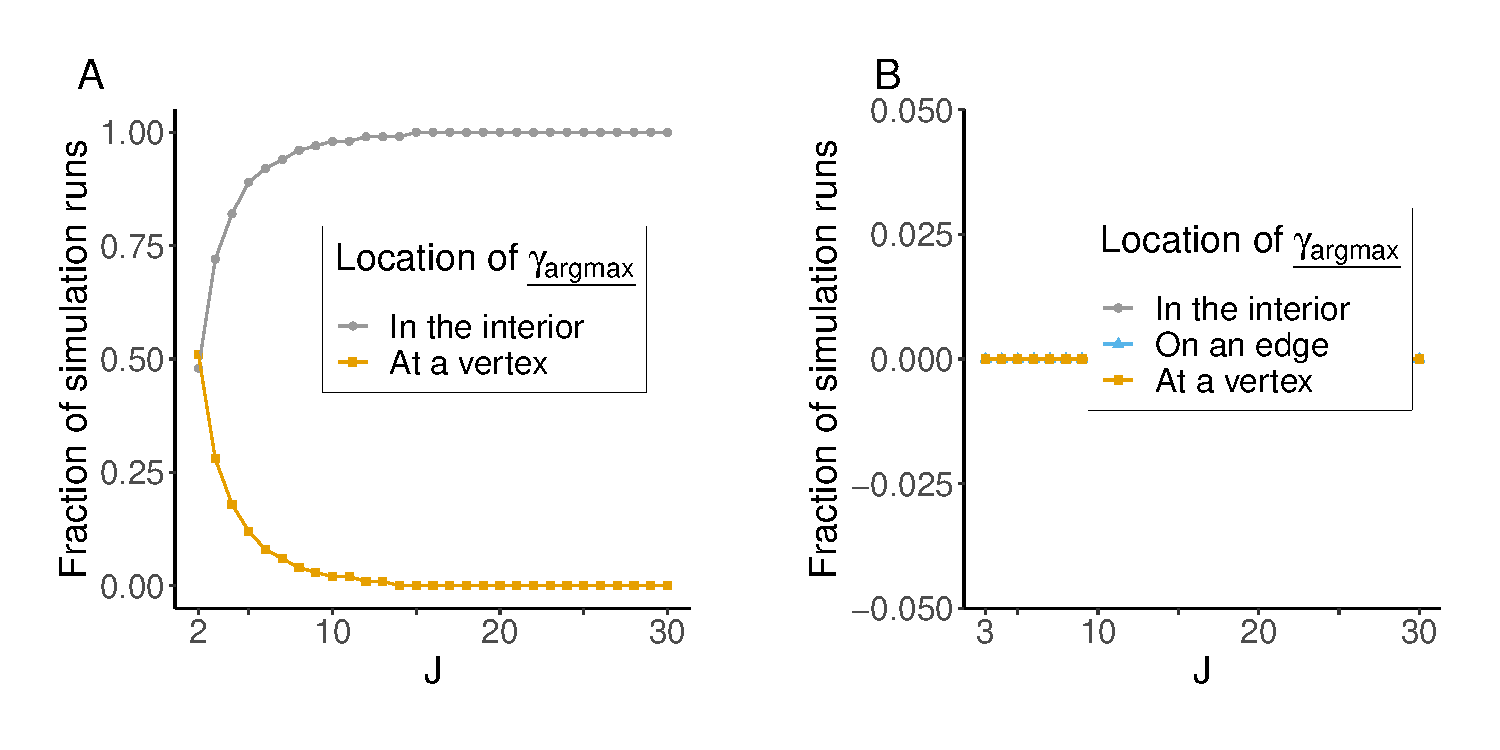
\includegraphics[width=\maxwidth]{../figs/Fig3-1} 

\end{knitrout}
